% Options for packages loaded elsewhere
\PassOptionsToPackage{unicode}{hyperref}
\PassOptionsToPackage{hyphens}{url}
%
\documentclass[
]{article}
\usepackage{amsmath,amssymb}
\usepackage{iftex}
\ifPDFTeX
  \usepackage[T1]{fontenc}
  \usepackage[utf8]{inputenc}
  \usepackage{textcomp} % provide euro and other symbols
\else % if luatex or xetex
  \usepackage{unicode-math} % this also loads fontspec
  \defaultfontfeatures{Scale=MatchLowercase}
  \defaultfontfeatures[\rmfamily]{Ligatures=TeX,Scale=1}
\fi
\usepackage{lmodern}
\ifPDFTeX\else
  % xetex/luatex font selection
\fi
% Use upquote if available, for straight quotes in verbatim environments
\IfFileExists{upquote.sty}{\usepackage{upquote}}{}
\IfFileExists{microtype.sty}{% use microtype if available
  \usepackage[]{microtype}
  \UseMicrotypeSet[protrusion]{basicmath} % disable protrusion for tt fonts
}{}
\makeatletter
\@ifundefined{KOMAClassName}{% if non-KOMA class
  \IfFileExists{parskip.sty}{%
    \usepackage{parskip}
  }{% else
    \setlength{\parindent}{0pt}
    \setlength{\parskip}{6pt plus 2pt minus 1pt}}
}{% if KOMA class
  \KOMAoptions{parskip=half}}
\makeatother
\usepackage{xcolor}
\usepackage[margin=1in]{geometry}
\usepackage{color}
\usepackage{fancyvrb}
\newcommand{\VerbBar}{|}
\newcommand{\VERB}{\Verb[commandchars=\\\{\}]}
\DefineVerbatimEnvironment{Highlighting}{Verbatim}{commandchars=\\\{\}}
% Add ',fontsize=\small' for more characters per line
\usepackage{framed}
\definecolor{shadecolor}{RGB}{248,248,248}
\newenvironment{Shaded}{\begin{snugshade}}{\end{snugshade}}
\newcommand{\AlertTok}[1]{\textcolor[rgb]{0.94,0.16,0.16}{#1}}
\newcommand{\AnnotationTok}[1]{\textcolor[rgb]{0.56,0.35,0.01}{\textbf{\textit{#1}}}}
\newcommand{\AttributeTok}[1]{\textcolor[rgb]{0.13,0.29,0.53}{#1}}
\newcommand{\BaseNTok}[1]{\textcolor[rgb]{0.00,0.00,0.81}{#1}}
\newcommand{\BuiltInTok}[1]{#1}
\newcommand{\CharTok}[1]{\textcolor[rgb]{0.31,0.60,0.02}{#1}}
\newcommand{\CommentTok}[1]{\textcolor[rgb]{0.56,0.35,0.01}{\textit{#1}}}
\newcommand{\CommentVarTok}[1]{\textcolor[rgb]{0.56,0.35,0.01}{\textbf{\textit{#1}}}}
\newcommand{\ConstantTok}[1]{\textcolor[rgb]{0.56,0.35,0.01}{#1}}
\newcommand{\ControlFlowTok}[1]{\textcolor[rgb]{0.13,0.29,0.53}{\textbf{#1}}}
\newcommand{\DataTypeTok}[1]{\textcolor[rgb]{0.13,0.29,0.53}{#1}}
\newcommand{\DecValTok}[1]{\textcolor[rgb]{0.00,0.00,0.81}{#1}}
\newcommand{\DocumentationTok}[1]{\textcolor[rgb]{0.56,0.35,0.01}{\textbf{\textit{#1}}}}
\newcommand{\ErrorTok}[1]{\textcolor[rgb]{0.64,0.00,0.00}{\textbf{#1}}}
\newcommand{\ExtensionTok}[1]{#1}
\newcommand{\FloatTok}[1]{\textcolor[rgb]{0.00,0.00,0.81}{#1}}
\newcommand{\FunctionTok}[1]{\textcolor[rgb]{0.13,0.29,0.53}{\textbf{#1}}}
\newcommand{\ImportTok}[1]{#1}
\newcommand{\InformationTok}[1]{\textcolor[rgb]{0.56,0.35,0.01}{\textbf{\textit{#1}}}}
\newcommand{\KeywordTok}[1]{\textcolor[rgb]{0.13,0.29,0.53}{\textbf{#1}}}
\newcommand{\NormalTok}[1]{#1}
\newcommand{\OperatorTok}[1]{\textcolor[rgb]{0.81,0.36,0.00}{\textbf{#1}}}
\newcommand{\OtherTok}[1]{\textcolor[rgb]{0.56,0.35,0.01}{#1}}
\newcommand{\PreprocessorTok}[1]{\textcolor[rgb]{0.56,0.35,0.01}{\textit{#1}}}
\newcommand{\RegionMarkerTok}[1]{#1}
\newcommand{\SpecialCharTok}[1]{\textcolor[rgb]{0.81,0.36,0.00}{\textbf{#1}}}
\newcommand{\SpecialStringTok}[1]{\textcolor[rgb]{0.31,0.60,0.02}{#1}}
\newcommand{\StringTok}[1]{\textcolor[rgb]{0.31,0.60,0.02}{#1}}
\newcommand{\VariableTok}[1]{\textcolor[rgb]{0.00,0.00,0.00}{#1}}
\newcommand{\VerbatimStringTok}[1]{\textcolor[rgb]{0.31,0.60,0.02}{#1}}
\newcommand{\WarningTok}[1]{\textcolor[rgb]{0.56,0.35,0.01}{\textbf{\textit{#1}}}}
\usepackage{graphicx}
\makeatletter
\def\maxwidth{\ifdim\Gin@nat@width>\linewidth\linewidth\else\Gin@nat@width\fi}
\def\maxheight{\ifdim\Gin@nat@height>\textheight\textheight\else\Gin@nat@height\fi}
\makeatother
% Scale images if necessary, so that they will not overflow the page
% margins by default, and it is still possible to overwrite the defaults
% using explicit options in \includegraphics[width, height, ...]{}
\setkeys{Gin}{width=\maxwidth,height=\maxheight,keepaspectratio}
% Set default figure placement to htbp
\makeatletter
\def\fps@figure{htbp}
\makeatother
\setlength{\emergencystretch}{3em} % prevent overfull lines
\providecommand{\tightlist}{%
  \setlength{\itemsep}{0pt}\setlength{\parskip}{0pt}}
\setcounter{secnumdepth}{-\maxdimen} % remove section numbering
\ifLuaTeX
  \usepackage{selnolig}  % disable illegal ligatures
\fi
\IfFileExists{bookmark.sty}{\usepackage{bookmark}}{\usepackage{hyperref}}
\IfFileExists{xurl.sty}{\usepackage{xurl}}{} % add URL line breaks if available
\urlstyle{same}
\hypersetup{
  pdftitle={Presentation},
  pdfauthor={Karrin Tennant},
  hidelinks,
  pdfcreator={LaTeX via pandoc}}

\title{Presentation}
\author{Karrin Tennant}
\date{2023-12-08}

\begin{document}
\maketitle

\begin{Shaded}
\begin{Highlighting}[]
\FunctionTok{setwd}\NormalTok{(}\StringTok{"C:/Users/karri/Documents/Night{-}Transpiration"}\NormalTok{)}
\NormalTok{knitr}\SpecialCharTok{::}\FunctionTok{include\_graphics}\NormalTok{(}\StringTok{"miscellaneous/pictures/thesis\_poster.png"}\NormalTok{)}
\end{Highlighting}
\end{Shaded}

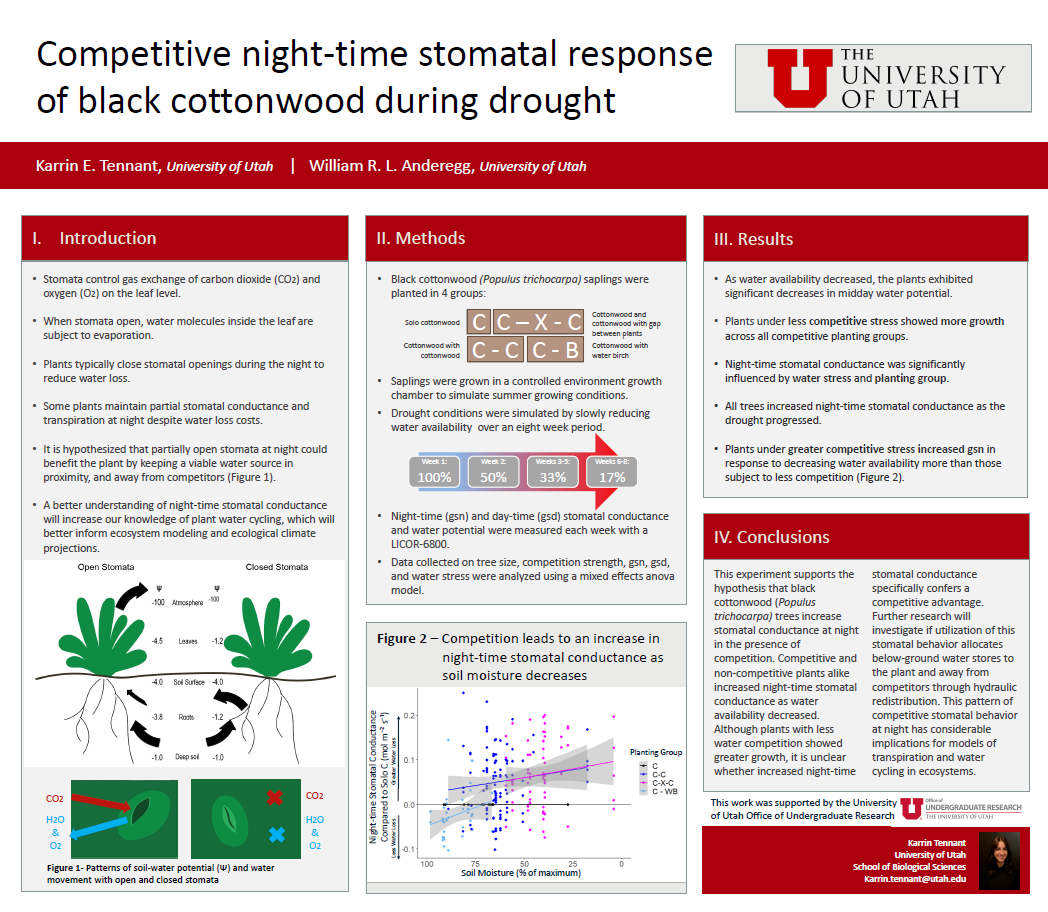
\includegraphics{miscellaneous/pictures/thesis_poster.png}

\hypertarget{repository-organization}{%
\subsection{Repository Organization}\label{repository-organization}}

\begin{Shaded}
\begin{Highlighting}[]
\ExtensionTok{tree}\NormalTok{ /mnt/c/Users/karri/Documents/Night{-}Transpiration}
\end{Highlighting}
\end{Shaded}

\begin{verbatim}
## /mnt/c/Users/karri/Documents/Night-Transpiration
## ├── LICENSE
## ├── README.md
## ├── data
## │   ├── processed_data
## │   │   ├── README.md
## │   │   ├── Transpiration.xlsx
## │   │   ├── bigdata.csv
## │   │   ├── bigdata_MD.csv
## │   │   ├── bigdata_PD.csv
## │   │   └── hegyi.xlsx
## │   └── raw_data
## │       ├── 2020-06-23-0943_pd.xlsx
## │       ├── 2020-06-23-1750_md.xlsx
## │       ├── 2020-06-24-0845_pd.xlsx
## │       ├── 2020-06-24-1751_md.xlsx
## │       ├── 2020-06-30-0902_pd.xlsx
## │       ├── 2020-06-30-1756_md.xlsx
## │       ├── 2020-07-02-0927_pd.xlsx
## │       ├── 2020-07-02-1802_md.xlsx
## │       ├── 2020-07-07-0917_pd.xlsx
## │       ├── 2020-07-07-1750_md.xlsx
## │       ├── 2020-07-08-0926_pd.xlsx
## │       ├── 2020-07-08-1758_md.xlsx
## │       ├── 2020-07-15-0856_pd.xlsx
## │       ├── 2020-07-15-1822_md.xlsx
## │       ├── 2020-07-22-0915_pd.xlsx
## │       ├── 2020-07-22-1713_md.xlsx
## │       ├── 2020-07-23-0915_pd.xlsx
## │       ├── 2020-07-23-1757_md.xlsx
## │       ├── 2020-08-01-0909_pd.xlsx
## │       ├── 2020-08-01-1756_md.xlsx
## │       ├── 2020-08-02-0831_pd.xlsx
## │       ├── 2020-08-02-1741_md.xlsx
## │       ├── 2020-08-05-0742_pd.xlsx
## │       ├── 2020-08-05-1714_md.xlsx
## │       ├── 2020-08-11-0836_pd.xlsx
## │       ├── 2020-08-11-1735_md.xlsx
## │       ├── 2020-08-18-0819_pd.xlsx
## │       ├── 2020-08-18-1739_md.xlsx
## │       ├── README.md
## │       ├── biomass.xlsx
## │       ├── growth.xlsx
## │       ├── metadata.xlsx
## │       └── soil.dat
## ├── experiment
## │   ├── README.md
## │   ├── analysis
## │   │   ├── README.md
## │   │   ├── anovas.R
## │   │   └── mixedfx.R
## │   ├── exploratory
## │   │   ├── README.md
## │   │   ├── gs_dataexploration.Rmd
## │   │   ├── gs_dataexploration.html
## │   │   └── gs_dataprocessing.html
## │   ├── figures
## │   │   ├── Fig1.tiff
## │   │   ├── Fig2.tiff
## │   │   ├── Fig3.tiff
## │   │   ├── Fig4.tiff
## │   │   ├── Fig5.tiff
## │   │   ├── Figure4.R
## │   │   ├── README.md
## │   │   ├── fig_gsn.tx.Rmd
## │   │   ├── fig_gsn.tx.html
## │   │   ├── figure9.R
## │   │   ├── greatgraphs.R
## │   │   └── mixedfx.R
## │   └── processing
## │       ├── README.md
## │       ├── functions.R
## │       ├── gs_dataprocessing.Rmd
## │       └── gs_dataprocessing.html
## ├── gsn.Rproj
## └── miscellaneous
##     ├── README.md
##     ├── manuscript
##     │   ├── 12.23Quantifying the effects of belowground intra- and inter-specific competition on nighttime stomatal conductance and transpiration in black cottonwoods.docx
##     │   └── README.md
##     ├── pictures
##     │   ├── IMG_0585.HEIC
##     │   ├── IMG_0586.HEIC
##     │   ├── IMG_0610.HEIC
##     │   ├── README.md
##     │   └── thesis_poster.png
##     └── protocols
##         ├── Class_presentation.Rmd
##         ├── Class_presentation.html
##         └── README.md
## 
## 12 directories, 77 files
\end{verbatim}

\hypertarget{process-raw-data}{%
\subsection{Process Raw Data}\label{process-raw-data}}

First, we import individual data files. Next, we combine them into a
master dataframe. Then, use functions stored in the `functions.R' script
to add columns populated by values based on conditional test.

\begin{Shaded}
\begin{Highlighting}[]
\FunctionTok{setwd}\NormalTok{(}\StringTok{"C:/Users/karri/Documents/Night{-}Transpiration"}\NormalTok{)}
\FunctionTok{source}\NormalTok{(}\StringTok{"experiment/processing/functions.R"}\NormalTok{)}
\end{Highlighting}
\end{Shaded}

\begin{Shaded}
\begin{Highlighting}[]
\FunctionTok{head}\NormalTok{(bigdata)}
\end{Highlighting}
\end{Shaded}

\begin{verbatim}
## # A tibble: 6 x 175
##     obs   time...2 elapsed date  hhmmss...5 species    ID TIME...8       E     A
##   <dbl>      <dbl>   <dbl> <chr> <chr>      <lgl>   <dbl>    <dbl>   <dbl> <dbl>
## 1     1     1.59e9      0  2020~ 17:56:12   NA         22   1.59e9 0.00355  9.89
## 2     2     1.59e9    176. 2020~ 17:59:08   NA         23   1.59e9 0.00636 18.6 
## 3     3     1.59e9    820. 2020~ 18:09:52   NA         24   1.59e9 0.00262  9.40
## 4     4     1.59e9    975. 2020~ 18:12:27   NA         25   1.59e9 0.00325 11.9 
## 5     5     1.59e9   1277. 2020~ 18:17:29   NA         26   1.59e9 0.00460  4.06
## 6     6     1.59e9   1497. 2020~ 18:21:09   NA         27   1.59e9 0.00617 11.1 
## # i 165 more variables: Ca <dbl>, Ci <dbl>, Pci <dbl>, Pca <dbl>, gsw <dbl>,
## #   gbw <dbl>, gtw <dbl>, gtc <dbl>, Rabs <dbl>, TleafEB <dbl>, TleafCnd <dbl>,
## #   SVPleaf <dbl>, RHcham <dbl>, VPcham <dbl>, SVPcham <dbl>, VPDleaf <dbl>,
## #   LatHFlux <dbl>, SenHFlux <dbl>, NetTherm <dbl>, EBSum <dbl>, Leak <dbl>,
## #   LeakPct <dbl>, CorrFact <dbl>, CorrFactPct <dbl>, Fan <dbl>, Qin <dbl>,
## #   Qabs <dbl>, alpha <dbl>, convert <dbl>, S <dbl>, K <dbl>, Geometry <chr>,
## #   Custom <dbl>, TIME...44 <dbl>, CO2_s <dbl>, CO2_r <dbl>, H2O_s <dbl>, ...
\end{verbatim}

\hypertarget{data-exploration}{%
\subsection{Data Exploration}\label{data-exploration}}

Explore processed data to visualize data distributions, summary
statistics, outliers, and variable co-linearity.

\begin{Shaded}
\begin{Highlighting}[]
\CommentTok{\# summary stats}
\FunctionTok{summary}\NormalTok{(bigdata}\SpecialCharTok{$}\NormalTok{gsw)}
\end{Highlighting}
\end{Shaded}

\begin{verbatim}
##     Min.  1st Qu.   Median     Mean  3rd Qu.     Max. 
## 0.003381 0.068865 0.141995 0.191191 0.289976 1.016324
\end{verbatim}

\begin{Shaded}
\begin{Highlighting}[]
\FunctionTok{summary}\NormalTok{(bigdata\_PD}\SpecialCharTok{$}\NormalTok{gsw)}
\end{Highlighting}
\end{Shaded}

\begin{verbatim}
##     Min.  1st Qu.   Median     Mean  3rd Qu.     Max. 
## 0.003381 0.051829 0.082158 0.094002 0.128038 0.303244
\end{verbatim}

\begin{Shaded}
\begin{Highlighting}[]
\FunctionTok{summary}\NormalTok{(bigdata\_MD}\SpecialCharTok{$}\NormalTok{gsw)}
\end{Highlighting}
\end{Shaded}

\begin{verbatim}
##    Min. 1st Qu.  Median    Mean 3rd Qu.    Max. 
## 0.00356 0.16930 0.28949 0.28838 0.39170 1.01632
\end{verbatim}

\begin{Shaded}
\begin{Highlighting}[]
\FunctionTok{summary}\NormalTok{(bigdata}\SpecialCharTok{$}\NormalTok{E)}
\end{Highlighting}
\end{Shaded}

\begin{verbatim}
##      Min.   1st Qu.    Median      Mean   3rd Qu.      Max. 
## 3.586e-05 1.488e-03 3.339e-03 4.153e-03 5.950e-03 1.652e-02
\end{verbatim}

\begin{Shaded}
\begin{Highlighting}[]
\FunctionTok{summary}\NormalTok{(bigdata\_PD}\SpecialCharTok{$}\NormalTok{E)}
\end{Highlighting}
\end{Shaded}

\begin{verbatim}
##      Min.   1st Qu.    Median      Mean   3rd Qu.      Max. 
## 3.586e-05 9.816e-04 1.703e-03 2.010e-03 2.922e-03 6.035e-03
\end{verbatim}

\begin{Shaded}
\begin{Highlighting}[]
\FunctionTok{summary}\NormalTok{(bigdata\_MD}\SpecialCharTok{$}\NormalTok{E)}
\end{Highlighting}
\end{Shaded}

\begin{verbatim}
##      Min.   1st Qu.    Median      Mean   3rd Qu.      Max. 
## 0.0001195 0.0040529 0.0059325 0.0062964 0.0080666 0.0165190
\end{verbatim}

\begin{Shaded}
\begin{Highlighting}[]
\FunctionTok{summary}\NormalTok{(bigdata}\SpecialCharTok{$}\NormalTok{A)}
\end{Highlighting}
\end{Shaded}

\begin{verbatim}
##    Min. 1st Qu.  Median    Mean 3rd Qu.    Max. 
## -5.8683 -1.0755 -0.1195  4.2344  9.6865 23.3797
\end{verbatim}

\begin{Shaded}
\begin{Highlighting}[]
\FunctionTok{summary}\NormalTok{(bigdata\_PD}\SpecialCharTok{$}\NormalTok{A)}
\end{Highlighting}
\end{Shaded}

\begin{verbatim}
##     Min.  1st Qu.   Median     Mean  3rd Qu.     Max. 
## -5.86833 -1.45707 -1.07537 -1.19175 -0.79611 -0.03236
\end{verbatim}

\begin{Shaded}
\begin{Highlighting}[]
\FunctionTok{summary}\NormalTok{(bigdata\_MD}\SpecialCharTok{$}\NormalTok{A)}
\end{Highlighting}
\end{Shaded}

\begin{verbatim}
##    Min. 1st Qu.  Median    Mean 3rd Qu.    Max. 
##  -1.169   6.466   9.698   9.660  12.449  23.380
\end{verbatim}

\begin{Shaded}
\begin{Highlighting}[]
\CommentTok{\#Check for normality/data distributions }
\NormalTok{op}\OtherTok{\textless{}{-}} \FunctionTok{par}\NormalTok{(}\AttributeTok{mfrow=}\FunctionTok{c}\NormalTok{(}\DecValTok{3}\NormalTok{,}\DecValTok{1}\NormalTok{))}
\FunctionTok{hist}\NormalTok{(bigdata}\SpecialCharTok{$}\NormalTok{gsw)}
\FunctionTok{hist}\NormalTok{(bigdata\_PD}\SpecialCharTok{$}\NormalTok{gsw)}
\FunctionTok{hist}\NormalTok{(bigdata\_MD}\SpecialCharTok{$}\NormalTok{gsw)}
\end{Highlighting}
\end{Shaded}

\includegraphics{Class_presentation_files/figure-latex/Data Exploration-1.pdf}

\begin{Shaded}
\begin{Highlighting}[]
\FunctionTok{hist}\NormalTok{(bigdata}\SpecialCharTok{$}\NormalTok{E)}
\FunctionTok{hist}\NormalTok{(bigdata\_PD}\SpecialCharTok{$}\NormalTok{E)}
\FunctionTok{hist}\NormalTok{(bigdata\_MD}\SpecialCharTok{$}\NormalTok{E)}
\end{Highlighting}
\end{Shaded}

\includegraphics{Class_presentation_files/figure-latex/Data Exploration-2.pdf}

\begin{Shaded}
\begin{Highlighting}[]
\FunctionTok{hist}\NormalTok{(bigdata}\SpecialCharTok{$}\NormalTok{A)}
\FunctionTok{hist}\NormalTok{(bigdata\_PD}\SpecialCharTok{$}\NormalTok{A)}
\FunctionTok{hist}\NormalTok{(bigdata\_PD}\SpecialCharTok{$}\NormalTok{A)}
\end{Highlighting}
\end{Shaded}

\includegraphics{Class_presentation_files/figure-latex/Data Exploration-3.pdf}

\begin{Shaded}
\begin{Highlighting}[]
\FunctionTok{par}\NormalTok{(op)}

\CommentTok{\#COLINEARITY{-}continuous variables}
\FunctionTok{select}\NormalTok{(bigdata, gsw,E,A) }\SpecialCharTok{\%\textgreater{}\%}
\FunctionTok{ggpairs}\NormalTok{() }
\end{Highlighting}
\end{Shaded}

\includegraphics{Class_presentation_files/figure-latex/Data Exploration-4.pdf}

\begin{Shaded}
\begin{Highlighting}[]
\FunctionTok{print}\NormalTok{(gs.boxplots, }\AttributeTok{width=}\FunctionTok{getOption}\NormalTok{(}\StringTok{"width"}\NormalTok{))}
\end{Highlighting}
\end{Shaded}

\includegraphics{Class_presentation_files/figure-latex/figure-1.pdf}

\begin{Shaded}
\begin{Highlighting}[]
\FunctionTok{setwd}\NormalTok{(}\StringTok{"C:/Users/karri/Documents/Night{-}Transpiration"}\NormalTok{)}
\NormalTok{knitr}\SpecialCharTok{::}\FunctionTok{include\_graphics}\NormalTok{(}\StringTok{"miscellaneous/pictures/IMG\_0610.HEIC"}\NormalTok{)}
\end{Highlighting}
\end{Shaded}

\includegraphics{miscellaneous/pictures/IMG_0610.HEIC}

\end{document}
